\documentclass[10pt, a4paper]{article}
\usepackage[DIV=14]{typearea}
% DIV defaults for A4 base
% font size: 10pt 11pt 12pt | DIV: 8 10 12

\usepackage{amsmath}
\usepackage{amsfonts}
\usepackage{amssymb}
\usepackage{physics}
\usepackage{bm}
\usepackage{graphicx}
\usepackage{enumitem}
\usepackage{xfrac}
\usepackage{extarrows}
\usepackage{float}
\usepackage{caption}
\usepackage{placeins}

\usepackage{polyglossia}
\setmainlanguage{spanish}
\setotherlanguage{english}

% =============================================================================
\usepackage{fontspec}

% =============================================================================
% ==========================================================================================
\RequirePackage{mathrsfs}
\RequirePackage{amsmath}
\RequirePackage{xparse}
\RequirePackage{physics}

% ==========================================================================================
\newcommand{\defeq}{\equiv}
\newcommand{\eqdef}{\defeq}

% ==========================================================================================
%\newcommand{\set}[1]{\left\{#1\right\}}
\newcommand{\set}[1]{\Bqty{#1}}                                         % dep. 'physics.sty'

% ==========================================================================================
%\newcommand{\vect}[1]{\bm{#1}}
%\newcommand{\vers}[1]{\vect{\hat{#1}}}
\newcommand{\vect}[1]{\vb*{#1}}                                         % dep. 'physics.sty'
\newcommand{\vers}[1]{\vu*{#1}}                                         % dep. 'physics.sty'

\newcommand{\conj}[1]{{{#1}^{*}}}

% ==========================================================================================
\newcommand{\Naturals}{\mathbb{N}}
\newcommand{\Integers}{\mathbb{Z}}
\newcommand{\Reals}{\mathbb{R}}
\newcommand{\Complex}{\mathbb{C}}

\newcommand{\Hilbert}{\mathscr{H}}

\newcommand{\lchivita}{\varepsilon}

% ==========================================================================================
\DeclareMathOperator{\Variance}{Var}
\DeclareMathOperator{\StandardDeviation}{Sdv}
\DeclareMathOperator{\Argument}{Arg}
\NewDocumentCommand{\Var}{}{\opbraces{\Variance}}                       % dep. 'physics.sty'
\NewDocumentCommand{\Sdv}{}{\opbraces{\StandardDeviation}}              % dep. 'physics.sty'
\NewDocumentCommand{\Arg}{}{\opbraces{\Argument}}                       % dep. 'physics.sty'
\NewDocumentCommand{\Fourier}{}{\opbraces{\mathcal{F}}}                 % dep. 'physics.sty'
\NewDocumentCommand{\TranslationOp}{}{\opbraces{\mathcal{T}}}           % dep. 'physics.sty'

\DeclareDocumentCommand\opsupscriptbraces{ m o d() }                    % dep. 'physics.sty'
{
	\IfNoValueTF{#3}
	{#1 \IfNoValueTF{#2}{}{[#2]}}
  {#1 \IfNoValueTF{#2}{}{^{\left(#2\right)}} \argopen(#3\argclose)}
}
\NewDocumentCommand{\RotationOp}{}{\opsupscriptbraces{\mathcal{D}}}     % dep. 'physics.sty'
\NewDocumentCommand{\RotationYMatrix}{}{\opsupscriptbraces{d}}          % dep. 'physics.sty'
\NewDocumentCommand{\SphericalHarmonic}{m m}{\opbraces{Y^{#2}_{#1}}}    % dep. 'physics.sty'

% ==========================================================================================
\newcommand{\Id}{\mathbb{I}}
\newcommand{\projector}[1]{\dyad{#1}}

\newcommand{\Prob}[1]{P\left({#1}\right)}
\newcommand{\ProbCond}[2]{P\left({#1}\middle|{#2}\right)}
\newcommand{\ProbRes}[2]{\ProbCond{#1}{#2}}
\newcommand{\HeisRepr}[1]{U^\dagger(t)\,{#1}\,U(t)}
\newcommand{\UnitConj}[2]{{#2}^\dagger\,{#1}\,{#2}}
\newcommand{\UnitConjPar}[2]{\left(#2\right)^\dagger\,{#1}\,\left(#2\right)}

\newcommand{\ketjm}[2]{\ket{j = {#1}, m = {#2}}}
\newcommand{\ketlm}[2]{\ket{l = {#1}, m = {#2}}}

\newcommand{\tensor}{\otimes}
\newcommand{\dirsum}{\oplus}

\newcommand{\doublebarmel}[3]{\left\langle{#1}\middle\|{#2}\middle\|{#3}\right\rangle}

\newcommand{\parityop}{\pi}
\newcommand{\translationop}{\mathcal{T}}

%\newcommand{\grad}{\vect{\nabla}}

%\newcommand{\order}[1]{\mathcal{O}\left(#1\right)}

% ==========================================================================================
\newcommand{\spin}{spin}
\newcommand{\spinhalf}{\spin~\ensuremath{1/2}}
\newcommand{\spinone}{\spin~\ensuremath{1}}

\newcommand{\TODO}[1]{{\small[\textbf{TO-DO}: {#1}]}}


\graphicspath{{./}{./images/}}

% =============================================================================
\usepackage[type={CC},modifier={by-nc-sa},version={4.0},lang={en}]{doclicense}

\usepackage[framemethod=tikz]{mdframed}
\mdfdefinestyle{mainframe}{
  frametitlebackgroundcolor=black!15,
  frametitlerule=true,
  roundcorner=10pt,
  middlelinewidth=1pt,
  innermargin=0.5cm,
  outermargin=0.5cm,
  innerleftmargin=0.5cm,
  innerrightmargin=0.5cm,
  innertopmargin=\topskip,
  innerbottommargin=\topskip,
}

% =============================================================================
\newcommand{\wt}{\omega t}

% Header ======================================================================
\usepackage{fancyhdr}
\usepackage{lastpage}
\fancyhead[L]{Apunte TPs Física Teórica 2: Dinámica}
\fancyhead[C]{}
\fancyhead[R]{\thepage/\pageref{LastPage}}
\fancyfoot{}
\renewcommand{\headrulewidth}{0.5pt}
\pagestyle{fancy}

\usepackage{titlesec}
%\renewcommand{\thesection}{\Roman{section}}
%\renewcommand{\thesubsection}{\Roman{subsection}}
\renewcommand{\thesubsubsection}{\Alph{subsubsection}}
%\titleformat{\section}{\large\bfseries\filcenter}{\Roman{section}.}{0.5em}{}
%\titleformat{\subsection}{\large\bfseries\filcenter}{\Roman{subsection}.}{0.5em}{}

\numberwithin{equation}{subsection}
\allowdisplaybreaks

\setcounter{tocdepth}{3}

% =============================================================================
\usepackage{hyperref}
\hypersetup{
    pdftitle={Apunte TPs Física Teórica 2: Dinámica},
    pdfauthor={Federico Cerisola},
    pdfencoding=auto,
    pdfstartview=Fit,
    pdfpagemode=UseOutlines,
    hypertexnames=false,
}

% =============================================================================
\begin{document}

% =============================================================================
\title{Apunte TPs Física Teórica 2: Dinámica}
\author{Federico Cerisola
  \\ \small{Departamento de Física -- FCEyN -- Universidad de Buenos Aires}
  \\ \small{\href{mailto:cerisola@df.uba.ar}{\nolinkurl{cerisola@df.uba.ar}}}
}
\date{\small Última actualización: \today}
\maketitle
\thispagestyle{empty}

\vfill
\doclicenseThis

\pagebreak

% =============================================================================
\newpage
  \tableofcontents
\newpage

% =============================================================================
\section{Representación de Schrödinger}

Como se vio en la teórica, la evolución temporal en Mecánica Cuántica está dada
por un operador unitario $U(t)$ que satisface la ecuación diferencial
\begin{equation} \label{eq:def_evol_temp_op}
  \pdv{t} U(t) = \frac{1}{i\hbar}H(t)U(t),
\end{equation}
donde $H(t)$ es el operador \emph{Hamiltoniano}, el \emph{observable}
correspondiente a la \emph{energía} del sistema. Así como clásicamente el
Hamiltoniano es el generador infinitesimal de las evoluciones temporales, en
cuántica identificaremos con Hamiltoniano (el observable energía) al generador
infinitesimal de las evoluciones temporales.

En la representación de Schrödinger, entenderemos la evolución temporal como
una evolución temporal del estado del sistema. En efecto, si inicialmente a $t
= 0$ el sistema se encuentra en un estado $\ket{\psi_0}$, entonces el estado
del sistema a tiempo $t$ será
\begin{equation}
  \ket{\psi(t)} = U(t)\ket{\psi_0}.
\end{equation}

Durante gran parte de la materia nos dedicaremos a estudiar sistemas cuyo
Hamiltoniano no depende explícitamente del tiempo, es decir
\begin{equation}
  \pdv{H}{t} = 0.
\end{equation}
Esta condición simplifica radicalmente el problema de la evolución temporal,
en cuanto la solución de la ecuación diferencial \eqref{eq:def_evol_temp_op} es
simplemente
\begin{equation}
  U(t) = e^{-\frac{it}{\hbar}H}.
\end{equation}
Como el operador $U(t)$ se puede escribir como una serie de potencias de $H$,
entonces, como vimos en la práctica de formalismo, necesariamente los
autoestados de $H$ también lo son de $U(t)$. Efectivamente, si
$\set{\ket{E_n}}$ es la base ortonormal de autoestados de $H$, es decir
\begin{equation}
  H\ket{E_n} = E_n\ket{E_n},
\end{equation}
entonces
\begin{equation} \label{eq:stat_states}
  U(t)\ket{E_n} = e^{-\frac{it}{\hbar}H}\ket{E_n} =
  e^{-\frac{it}{\hbar}E_n}\ket{E_n}.
\end{equation}
Notar que, como las fases globales son irrelevantes para el cálculo de
probabilidades y valores medios, entonces los autoestados del Hamiltoniano
básicamente no evolucionan en el tiempo (son estados \emph{estacionarios}).
En particular, las probabilidades calculadas en estos estados no dependen del
tiempo (y por lo tanto tampoco los valores medios). En efecto, la probabilidad
de medir un resultado cuyo autoestado es $\ket{a}$ en función del tiempo es
\begin{equation}
  P(a|t) = \abs{\braket{a}{E_n(t)}}^2 = \abs{\matrixel{a}{U(t)}{E_n}}^2 =
    \abs{\matrixel{a}{e^{-\frac{it}{\hbar}E_n}}{E_n}}^2 =
    \abs{e^{-\frac{it}{\hbar}E_n}\braket{a}{E_n}}^2 =
    \abs{\braket{a}{E_n}}^2 = P(a|t = 0).
\end{equation}

\bigbreak

La ecuación \eqref{eq:stat_states} nos muestra que la evolución temporal de
estados para el caso de Hamiltonianos independientes del tiempo es un problema
trivial y siempre se puede resolver de la siguiente forma:

\begin{mdframed}[style=mainframe,
  frametitle={Evolución temporal de estados [dim. finita, $H$ indep. tiempo]}]
  Dado un sistema cuántico de dimensión finita, un estado inicial
  $\ket{\psi_0}$ y un Hamiltoniano $H$ (independiente del tiempo), para
  calcular el estado a tiempo $t$, $\ket{\psi(t)}$, siempre podemos proceder de
  la siguiente forma:
  \begin{enumerate}
    \item Diagonalizamos el Hamiltoniano $H$, encontrando sus autoestados
      ($\set{\ket{E_n}}$) y autovalores ($\set{E_n}$),
      \begin{equation}
        H\ket{E_n} = E_n\ket{E_n}.
      \end{equation}
      Luego,
      \begin{equation}
        U(t)\ket{E_n} = e^{-\frac{it}{\hbar}H}\ket{E_n} =
        e^{-\frac{it}{\hbar}E_n}\ket{E_n}.
      \end{equation}
    \item Escribimos el estado inicial, $\ket{\psi_0}$, en la base de
      autoestados de $H$,
      \begin{equation}
        \ket{\psi_0} = \sum_{n}\braket{E_n}{\psi_0}\ket{E_n} =
        \sum_{n}c_n\ket{E_n},
      \end{equation}
      con $c_n = \braket{E_n}{\psi_0}$.
    \item Finalmente, la evolución temporal es simplemente
      \begin{equation}
        \ket{\psi(t)} = U(t)\ket{\psi_0} = \sum_{n}c_nU(t)\ket{E_n} =
        \sum_{n}c_ne^{-\frac{it}{\hbar}E_n}\ket{E_n} =
        \sum_{n}c_n(t)\ket{E_n},
      \end{equation}
      con $c_n(t) = c_ne^{-\frac{it}{\hbar}E_n} =
      \braket{E_n}{\psi_0}e^{-\frac{it}{\hbar}E_n}$.
  \end{enumerate}
\end{mdframed}

% -----------------------------------------------------------------------------
\subsection{Problema 2 (Guía 4): Precesión del \spin}

Como primer ejemplo, veremos el problema de la precesión del \spin\ en un campo
magnético. El Hamiltoniano de interacción del grado de libertad de \spinhalf\
de un electrón en presencia de un campo magnético $B$ estático y uniforme que
apunta en la dirección $\vers{z}$ es
\begin{equation}
  H = \omega S_z,
\end{equation}
con $\omega = \abs{e}B/m$, con $\abs{e}$ la carga del electrón, $B$ la amplitud
del campo magnético, $m$ la masa del electrón y $S_z$ el operador de \spin\ en
la dirección $\vers{z}$ (ver enunciado Problema 2 -- Guía 4 para una
explicación de cómo se llega a este Hamiltoniano). Recordando que para un
\spinhalf,
\begin{equation}
  S_j = \frac{\hbar}{2}\sigma_j, \quad\left(j = x, y, z\right),
\end{equation}
con $\sigma_j$ la correspondiente matriz de Pauli, podemos finalmente escribir
el Hamiltoniano como
\begin{equation}
  H = \frac{\hbar\omega}{2}\sigma_z.
\end{equation}

Por lo tanto, los autoestados del Hamiltoniano son los autoestados de
$\sigma_z$, que denotamos como $\set{\ket{+}, \ket{-}}$ y tienen autovalores
para $\sigma_z$ $+1$ y $-1$ respectivamente. Efectivamente tenemos que
\begin{equation}
  H\ket{\pm} = \frac{\hbar\omega}{2}\sigma_z\ket{\pm} =
  \pm\frac{\hbar\omega}{2}\ket{\pm}.
\end{equation}
Por lo tanto, como nos sugieren en el ítem \textbf{(a)} del problema, los
autoestados del Hamiltoniano son los estados $\set{\ket{+}, \ket{-}}$, con
energías respectivas $\{E_+ = \frac{\hbar\omega}{2}, E_- =
-\frac{\hbar\omega}{2}\}$.

\bigbreak

En el ítem \textbf{(b)} nos dicen que inicialmente el sistema se encuentra en
el estado con \spin\ $+\hbar/2$ en la dirección $\vers{x}$, es decir que
inicialmente se encuentra en el autoestado de $S_x$ con autovalor $+\hbar/2$ o,
equivalentemente, en el autoestado de la matriz de Pauli $\sigma_x$ con
autovalor $+1$, que denotamos $\ket{+,\vers{x}}$. Para calcular la evolución
temporal del estado, siguiendo el procedimiento antes delineado, buscamos
escribir el estado inicial en la base de autoestados de $H$. En la base
$\set{\ket{+}, \ket{-}}$ de autoestados de $\sigma_z$, la matriz de Pauli
$\sigma_x$ se escribe como
\begin{equation} \label{eq:def_paulix}
  \sigma_x = \begin{pmatrix} 0 & 1 \\ 1 & 0 \end{pmatrix}.
\end{equation}
Diagonalizando la matriz tenemos que el autoestado $\ket{+,\vers{x}}$ está dado
por
\begin{equation}
  \ket{+,\vers{x}} = \frac{1}{\sqrt{2}}\left(\ket{+} + \ket{-}\right).
\end{equation}
Por lo tanto, el estado inicial en la base de autoestados de energía se escribe
como
\begin{equation} \label{eq:spinevol_ini_state}
  \ket{\psi(0)} = \ket{+,\vers{x}} =
  \frac{1}{\sqrt{2}}\left(\ket{+} + \ket{-}\right).
\end{equation}

Finalmente, el estado evolucionado un tiempo $t$ es
\begin{align}
  \ket{\psi(t)} &= U(t)\ket{\psi(0)}
    = e^{-\frac{it}{\hbar}H}\ket{\psi(0)}
    = e^{-\frac{i\wt}{2}\sigma_z}\ket{\psi(0)} \nonumber \\
  &= e^{-\frac{i\wt}{2}\sigma_z}
    \frac{1}{\sqrt{2}}\left(\ket{+} + \ket{-}\right) \nonumber \\
  &= \frac{1}{\sqrt{2}}\left(e^{-\frac{i\wt}{2}}\ket{+} +
    e^{+\frac{i\wt}{2}}\ket{-} \right). \label{eq:spinevol_t_state}
\end{align}

\bigbreak

En el ítem \textbf{(c)} nos piden calcular la probabilidad de obtener los
resultados $+\hbar/2$ y $-\hbar/2$ si se mide $S_x$ a un tiempo $t$. Para ello,
como es usual, escribimos el estado $\ket{\psi(t)}$ en la base de autoestados
de $S_x = (\hbar/2)\sigma_x$. Diagonalizando $\sigma_x$ (definido en
\eqref{eq:def_paulix}) tenemos los estados
\begin{align}
  \ket{\pm,\vers{x}} &= \frac{1}{\sqrt{2}}\left(\ket{+} \pm \ket{-}\right),\\
  S_x\ket{\pm,\vers{x}} &= \pm\frac{\hbar}{2}\ket{\pm,\vers{x}}.
\end{align}

Por lo tanto, la probabilidad de obtener los resultados $\pm\hbar/2$ al medir
$S_x$ a tiempo $t$ está dada por
\begin{equation}
  \ProbRes{\pm\frac{\hbar}{2},\vers{x}}{\psi(t)} =
  \abs{\braket{\pm,\vers{x}}{\psi(t)}}^2.
\end{equation}

Para el caso $+\hbar/2$ tenemos
\begin{align}
  \braket{+,\vers{x}}{\psi(t)} &=
    \left(\frac{1}{\sqrt{2}}\left(\bra{+} + \bra{-}\right)\right)
    \left(\frac{1}{\sqrt{2}}\left(e^{-\frac{i\wt}{2}}\ket{+} +
                                  e^{ \frac{i\wt}{2}}\ket{-}
    \right)\right) \\
  &= \frac{1}{2}\left(
    e^{-\frac{i\wt}{2}}\underbrace{\braket{+}{+}}_{1} +
    e^{-\frac{i\wt}{2}}\underbrace{\braket{-}{+}}_{0} +
    e^{ \frac{i\wt}{2}}\underbrace{\braket{+}{-}}_{0} +
    e^{ \frac{i\wt}{2}}\underbrace{\braket{-}{-}}_{1}
  \right) \\
  &= \frac{1}{2}\left(
    e^{-\frac{i\wt}{2}} +
    e^{ \frac{i\wt}{2}}
  \right) \\
  &= \cos\left(\frac{\wt}{2}\right).
\end{align}
Por lo tanto, la correspondiente probabilidad es
\begin{equation}
  \ProbRes{+\frac{\hbar}{2},\vers{x}}{\psi(t)} =
  \abs{\braket{+,\vers{x}}{\psi(t)}}^2 =
  \cos^2\left(\frac{\wt}{2}\right).
\end{equation}

Por otro lado, para $-\hbar/2$ tenemos
\begin{align}
  \braket{-,\vers{x}}{\psi(t)} &=
    \left(\frac{1}{\sqrt{2}}\left(\bra{+} - \bra{-}\right)\right)
    \left(\frac{1}{\sqrt{2}}\left(e^{-\frac{i\wt}{2}}\ket{+} +
                                  e^{ \frac{i\wt}{2}}\ket{-}
    \right)\right) \\
  &= \frac{1}{2}\left(
    e^{-\frac{i\wt}{2}}\underbrace{\braket{+}{+}}_{1} -
    e^{-\frac{i\wt}{2}}\underbrace{\braket{-}{+}}_{0} +
    e^{ \frac{i\wt}{2}}\underbrace{\braket{+}{-}}_{0} -
    e^{ \frac{i\wt}{2}}\underbrace{\braket{-}{-}}_{1}
  \right) \\
  &= \frac{1}{2}\left(
    e^{-\frac{i\wt}{2}} -
    e^{ \frac{i\wt}{2}}
  \right) \\
  &= i\sin\left(\frac{\wt}{2}\right).
\end{align}
Por lo tanto, la correspondiente probabilidad es
\begin{equation}
  \ProbRes{-\frac{\hbar}{2},\vers{x}}{\psi(t)} =
  \abs{\braket{-,\vers{x}}{\psi(t)}}^2 =
  \sin^2\left(\frac{\wt}{2}\right).
\end{equation}

Como siempre, esto es equivalente a escribir el estado $\ket{\psi(t)}$ en la
base de autoestados de $S_x$ y después simplemente obtener las probabilidades 
como módulos cuadrados de las amplitudes de los coeficientes de los
correspondientes autovectores. Efectivamente, $\ket{\psi(t)}$ en la base $S_x$
es
\begin{equation}
  \ket{\psi(t)} = \braket{+,\vers{x}}{\psi(t)}\ket{+,\vers{x}} +
                  \braket{-,\vers{x}}{\psi(t)}\ket{-,\vers{x}}.
\end{equation}
Usando los resultados del cálculos de los coeficientes
$\braket{\pm,\vers{x}}{\psi(t)}$ tenemos
\begin{equation} \label{eq:tevol_spinevol_sx_basis}
  \ket{\psi(t)} = \cos\left(\frac{\wt}{2}\right)\ket{+,\vers{x}} +
                 i\sin\left(\frac{\wt}{2}\right)\ket{-,\vers{x}}.
\end{equation}
Finalmente las probabilidades de los resultados $\ket{\pm,\vers{x}}$ son,
respectivamente, $\cos^2(\wt/2)$ y $\sin^2(\wt/2)$.

\begin{figure}[tb]
  \centering
  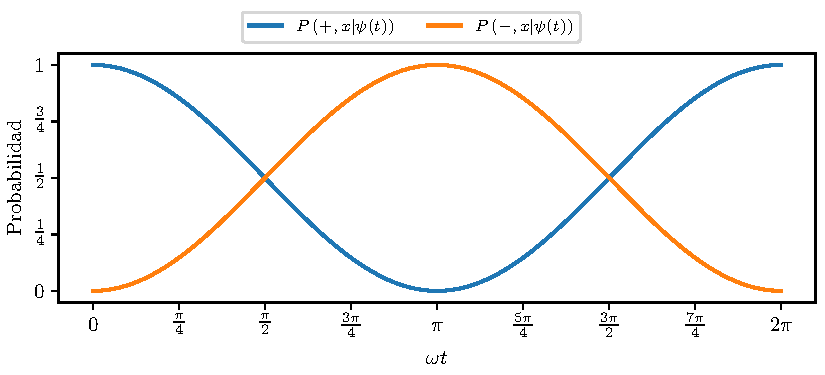
\includegraphics{images/spinevol_prob_sx.pdf}
  \caption{Probabilidad de obtener los resultados $\pm\hbar/2$ al medir $S_x$
    en función del tiempo.\label{fig:prob_sx_t}}
\end{figure}

En la figura \ref{fig:prob_sx_t} se muestra el gráfico de las probabilidades de
obtener los resultados $\pm\hbar/2$ al medir $S_x$ en función del tiempo. Se
observa que las probabilidades oscilan con un período $T = 2\pi / \omega$. En
particular, son notables los tiempo $(\pi/2)/\omega$ y $(3\pi/2)\omega$ donde
ambos resultados son equiprobables y el tiempo $\pi / \omega$ donde la
probabilidad de medir el resultado $+\hbar/2$ es 1, lo cual indica que a este
tiempo el estado es $\ket{\psi(\pi/\omega)} = \ket{-,\vers{x}}$ (esto
efectivamente se puede ver en la ecuación \eqref{eq:tevol_spinevol_sx_basis}).

\bigbreak

En el ítem \textbf{(d)} nos piden calcular los valores medios $\expval{S_x}$,
$\expval{S_y}$ y $\expval{S_z}$ en función del tiempo. Por definición, sabemos
que
\begin{equation} \label{eq:def_expval}
  \expval{S_j}(t) = \expval{S_j}{\psi(t)}, \quad\left(j = x,y,z\right).
\end{equation}

Sin embargo, notar que para el caso de $S_x$, como ya calculamos las
probabilidades de obtener los resultados $\pm\hbar/2$ en el ítem \textbf{(c)},
no hace falta hacer la cuenta anterior, sino que simplemente podemos usar que
\begin{equation}
  \expval{S_x}(t) = \left(\frac{\hbar}{2}\right)\ProbRes{+,\vers{x}}{\psi(t)}
                 + \left(-\frac{\hbar}{2}\right)\ProbRes{-,\vers{x}}{\psi(t)}
                  = \frac{\hbar}{2}\left[\ProbRes{+,\vers{x}}{\psi(t)} -
                    \ProbRes{-,\vers{x}}{\psi(t)}\right].
\end{equation}
(recordar que, como mostramos en las guías anteriores, las definiciones de cómo
calcular probabilidades y valores medios son consistentes de forma tal que esto
efectivamente siempre es cierto).
Por lo tanto,
\begin{equation} \label{eq:spinevol_expval_sx}
  \expval{S_x}(t) = \frac{\hbar}{2}\left[\cos^2\left(\frac{\wt}{2}\right) -
                    \sin^2\left(\frac{\wt}{2}\right)\right]
                  = \frac{\hbar}{2}\cos\wt.
\end{equation}

Para calcular $\expval{S_y}$ a partir de \eqref{eq:def_expval} usamos que $S_y
= (\hbar/2)\sigma_y$ y $\sigma_y$ en la base $\set{\ket{+}, \ket{-}}$ se
escribe
\begin{equation}
  \sigma_y = \begin{pmatrix} 0 & -i \\ i & 0 \end{pmatrix}.
\end{equation}

Por lo tanto,
\begin{equation}
  \sigma_y\ket{+} = i\ket{-}, \qquad \sigma_y\ket{-} = -i\ket{+}.
\end{equation}

\begin{figure}[tb]
  \centering
  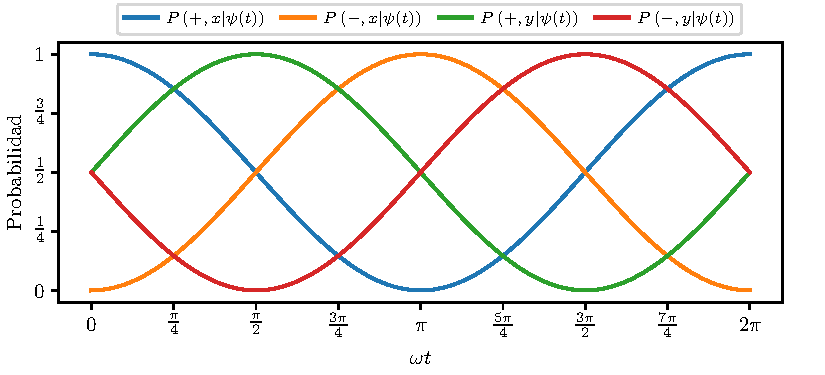
\includegraphics{images/spinevol_prob_sxsy.pdf}
  \caption{Probabilidad de obtener los resultados $\pm\hbar/2$ al medir $S_x$ y
    $S_y$ en función del tiempo.\label{fig:prob_sxsy_t}}

  \vspace*{\floatsep}% https://tex.stackexchange.com/q/26521/5764

  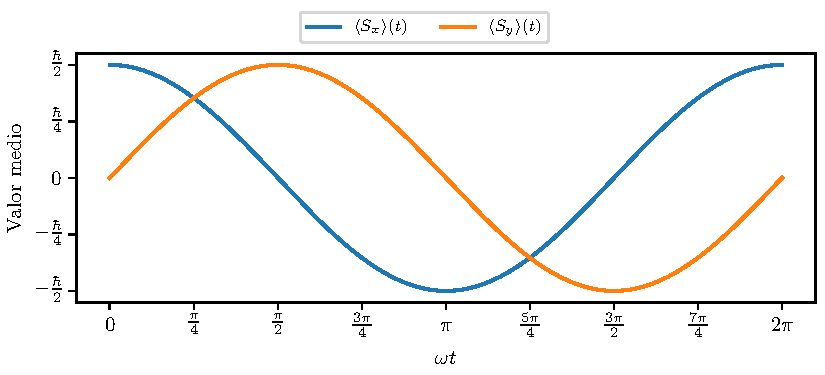
\includegraphics{images/spinevol_expval_sxsy.pdf}
  \caption{Valores medios de $S_x$ y $S_y$ en función del
    tiempo.\label{fig:expval_sxsy_t}}
\end{figure}

Entonces,
\begin{align}
  S_y\ket{\psi(t)} &= \frac{1}{\sqrt{2}}
    \left(e^{-\frac{i\wt}{2}}S_y\ket{+} + e^{+\frac{i\wt}{2}}S_y\ket{-}\right)
    \nonumber \\
  &= \frac{\hbar}{2}\frac{1}{\sqrt{2}}
    \left(e^{-\frac{i\wt}{2}}i\ket{-} + e^{+\frac{i\wt}{2}}(-i)\ket{+}\right)
    \nonumber \\
  &= \frac{i\hbar}{2\sqrt{2}}
    \left(e^{-\frac{i\wt}{2}}\ket{-} - e^{+\frac{i\wt}{2}}\ket{+}\right)
\end{align}

Finalmente,
\begin{align}
  \expval{S_y} &= \expval{S_y}{\psi(t)}
    = \bra{\psi(t)}\left(\frac{i\hbar}{2\sqrt{2}}
    \left(e^{-\frac{i\wt}{2}}\ket{-} - e^{\frac{i\wt}{2}}\ket{+}\right)\right)
    \nonumber \\
  &= \left(\frac{1}{\sqrt{2}}\left(e^{\frac{i\wt}{2}}\bra{+} +
    e^{-\frac{i\wt}{2}}\bra{-}\right) \right) \left(\frac{i\hbar}{2\sqrt{2}}
    \left(e^{-\frac{i\wt}{2}}\ket{-} - e^{\frac{i\wt}{2}}\ket{+}\right)\right)
    \nonumber \\
  &= \frac{i\hbar}{4} \left(-e^{i\wt} + e^{-i\wt}\right)
    \nonumber \\
  &= \frac{\hbar}{2} \sin\wt. \label{eq:spinevol_expval_sy}
\end{align}

Solamente quedaría calcular el valor medio de $S_z$. Sin embargo, notemos que
$\comm{S_z}{H} = 0$ (en particular en este caso $H \propto S_z$). Como se vio
en la teórica, cuando un operador conmuta con el Hamiltoniano, las
probabilidades de medir los distintos resultados son constantes en el tiempo (y
por lo tanto también lo es el valor medio). Luego, $\expval{S_z}(t) =
\expval{S_z}(0) = 0$, dado que el estado inicial es
\eqref{eq:spinevol_ini_state}.

En la figura \ref{fig:expval_sxsy_t} se muestra el gráfico de los valores
medios $\expval{S_x}$ y $\expval{S_y}$ en función del tiempo. Por otro lado, en
la figura \ref{fig:prob_sxsy_t} se muestra los gráficos de las probabilidades
de obtener $\pm\hbar/2$ al medir $S_x$ (que ya calculamos antes) o $S_y$ (que
el ejercicio no pide pero acá incluyo por completitud; les queda a ustedes
verificar si quieren que $\ProbRes{+,\vers{y}}{\psi(t)} = \sin^2(\wt/2 +
\pi/4)$ y $\ProbRes{-,\vers{y}}{\psi(t)} = \cos^2(\wt/2 + \pi/4)$).

\bigbreak

En la figura \ref{fig:prob_sxsy_t} de las probabilidades en función del tiempo
vemos que en los tiempos $(\pi/2)\omega$ y $(3\pi/2)/\omega$, donde teníamos
que $P(+,\vers{x}) = P(-,\vers{x}) = 1/2$, efectivamente tenemos probabilidad 1
de tener el estado $\ket{+,\vers{y}}$ o $\ket{-,\vers{y}}$, respectivamente.
Efectivamente, como ya habíamos visto en guías anteriores, cuando estamos en un
autoestado de \spin\ en una dirección, tenemos incerteza total en las
mediciones de \spin\ en cualquier dirección ortogonal. La figura
\ref{fig:prob_sxsy_t} de las probabilidades nos da además una buena idea de qué
le está sucediendo al sistema. Notemos que comenzamos a $t = 0$ en el estado
$\ket{+,\vers{x}}$. Luego a tiempo $t = (\pi/2)\omega$ estamos en el estado
$\ket{+,\vers{y}}$. A tiempo $t = \pi/\omega$ pasamos al estado
$\ket{-,\vers{x}}$. Luego a $t = (3\pi/2)/\omega$ alcanzamos el estado
$\ket{-,\vers{y}}$ y finalmente a $t = 2\pi/\omega$ volvemos al estado inicial
y el ciclo se repite. Por lo tanto, es como si el estado estuviese rotando
alrededor del eje $\vers{z}$ (dirección del campo magnético) y alternándose
entre autoestados de $S_x$ y $S_y$. Quizás no queda todavía del todo claro qué
pasa en los tiempos intermedios y cómo podemos interpretar el estado del
sistema $\ket{\psi(t)}$ a todo tiempo. Para terminar de entender cómo está
evolucionando el sistema, resulta extremadamente útil utilizar la
representación en la esfera de Bloch.

\bigbreak

\begin{figure}
  \begin{minipage}[t]{0.5\textwidth}
    \vspace{0pt}
    %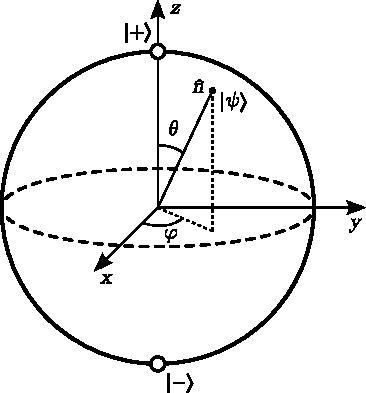
\includegraphics[width=0.85\linewidth]{images/Bloch_sphere_spinhalf.pdf}
    \def\svgwidth{0.85\linewidth}
    \input{images/Bloch_sphere_spinhalf_v2.pdf_tex}
  \end{minipage}%
  \begin{minipage}[t]{0.5\textwidth}
    \vspace{10pt}
    \captionof{figure}{Representación en la esfera de Bloch. Al estado
      $\ket{\psi} = \cos(\theta/2)\ket{+} + e^{i\varphi}\sin(\theta/2)\ket{-}$
      le corresponde el versor $\vers{n}(\theta, \varphi) =
      \left(\sin\theta\cos\varphi, \sin\theta\sin\varphi, \cos\theta\right)$
      con ángulos polares $\theta$ y $\varphi$.}
    \label{fig:def_bloch}
  \end{minipage}
\end{figure}

Recordemos que la idea detrás de la representación de la esfera de Bloch es
que, todo vector $\ket{\Psi}$ de un espacio de Hilbert complejo de dimensión 2,
normalizado y definido a menos de una fase global, siempre se puede escribir
como
\begin{equation} \label{eq:def_psi_bloch}
  \ket{\Psi} = \cos\frac{\theta}{2}\ket{+} +
  e^{i\varphi}\sin\frac{\theta}{2}\ket{-},
  \qquad\theta\in\left[0,\pi\right],\;\varphi\in\left[0,2\pi\right].
\end{equation}

Luego, es simplemente cuestión de darse cuenta que todo versor unitario
$\vers{n}$ en $\Reals^3$ (es decir todo punto de $\Reals^3$ sobre una esfera de
radio 1) se puede parametrizar en coordenadas polares como
\begin{equation}
  \vers{n} = \left(\sin\theta\cos\varphi, \sin\theta\sin\varphi,
  \cos\theta\right),
  \qquad\theta\in\left[0,\pi\right],\;\varphi\in\left[0,2\pi\right].
\end{equation}

Por lo tanto tenemos una relación 1 a 1,
\begin{equation}
  \ket{\Psi(\theta,\varphi)}
  \xlongleftrightarrow{\text{  1 a 1  }}
  \vers{n}(\theta,\varphi).
\end{equation}
En la figura \ref{fig:def_bloch} se muestra gráficamente la correspondencia del
estado $\ket{\Psi(\theta,\varphi)}$ con un punto sobre la esfera de Bloch.

\bigbreak

En nuestro caso, el estado a tiempo $t$ es \eqref{eq:spinevol_t_state}. Para
llevarlo a la forma de la ecuación \eqref{eq:def_psi_bloch} podemos sacar a
factor común una fase global
\begin{equation}
  \ket{\psi(t)} = \frac{1}{\sqrt{2}} e^{-\frac{i\wt}{2}}
    \left(\ket{+} + e^{i\wt}\ket{-}\right).
\end{equation}
A menos de una fase global, este estado es equivalente al estado
\begin{equation}
  \ket{\psi(t)} \cong \frac{1}{\sqrt{2}}
    \left(\ket{+} + e^{i\wt}\ket{-}\right).
\end{equation}
Por lo tanto, los respectivos ángulos polares $\theta(t)$ y $\varphi(t)$ son
\begin{equation}
  \theta(t) = \frac{\pi}{2}, \quad \varphi(t) = \wt.
\end{equation}

% old pos fig spin-bloch-tevol-equ

\begin{figure}
  \centering
  \begin{minipage}{.5\textwidth}
    \centering
    %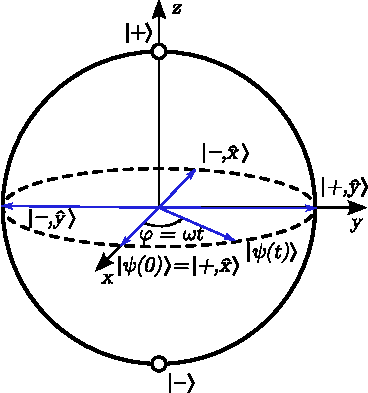
\includegraphics[width=0.85\linewidth]{images/Bloch_sphere_spinhalf_tevol_equ.pdf}
    \def\svgwidth{0.85\linewidth}
    \input{images/Bloch_sphere_spinhalf_tevol_equ_v2.pdf_tex}
  \end{minipage}%
  \begin{minipage}{.5\textwidth}
    \centering
    %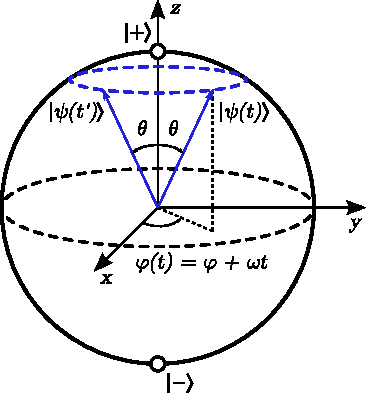
\includegraphics[width=0.85\linewidth]{images/Bloch_sphere_spinhalf_tevol_gen.pdf}
    \def\svgwidth{0.85\linewidth}
    \input{images/Bloch_sphere_spinhalf_tevol_gen_v2.pdf_tex}
  \end{minipage}
  \par
  \medskip
  \noindent
  \begin{minipage}[t]{.49\textwidth}
    \centering
    \captionof{figure}{Representación en la esfera de Bloch de la evolución
      temporal del estado inicial $\ket{\psi(0)} = \ket{+,\vers{x}}$. El estado
      rota alrededor del eje $\vers{z}$ con velocidad angular $\omega$,
      manteniéndose en el ecuador de la esfera. El ángulo azimutal varía como
      $\varphi(t) = \wt$.}
    \label{fig:bloch_tevol_equ}
  \end{minipage}%
  \hfill
  \begin{minipage}[t]{.49\textwidth}
    \centering
    \captionof{figure}{Representación en la esfera de Bloch de la evolución
      temporal del estado inicial más general $\ket{\psi(0)} =
      \cos(\theta/2)\ket{+} + e^{i\varphi}\sin(\theta/2)\ket{-}$. El estado
      rota alrededor del eje $\vers{z}$ con velocidad angular $\omega$,
      manteniéndose con un ángulo $\theta$ constante respecto del eje
      $\vers{z}$. En ángulo azimutal varía como $\varphi(t) = \varphi + \wt$.}
    \label{fig:bloch_tevol_gen}
  \end{minipage}
\end{figure}

En la figura \ref{fig:bloch_tevol_equ} se muestra el gráfico del estado
$\ket{\psi(t)}$ a distintos tiempos en la esfera de Bloch. Notemos primero que
$\theta(t) = \pi/2$ permanece constante en el tiempo y, por lo tanto, el estado
$\ket{\psi(t)}$ se encuentra siempre sobre el ecuador de la esfera. Por otro
lado, el ángulo azimutal varía como $\varphi(t) = \wt$. Por lo tanto, vemos que
efectivamente el estado del sistema rota alrededor del eje $\vers{z}$
(dirección del campo magnético) con velocidad angular $\omega$. Es más,
recordemos que en la guía de sistemas de dimensión 2 mostramos que el estado
\eqref{eq:def_psi_bloch} es autoestado del operador de \spin\ en la dirección
$\vers{n}(\theta,\varphi)$, $\vect{S}\cdot\vers{n}(\theta,\varphi)$. Por lo
tanto, tenemos una interpretación tiempo a tiempo del estado del sistema.
Comenzando en el autoestado $+\hbar/2$ de $S_x$, el estado del sistema rota
alrededor del eje $\vers{z}$, siendo tiempo a tiempo autoestado $+\hbar/2$ del
\spin\ en la dirección $\vers{n}(t)$ con $\theta(t) = \pi/2$ y $\varphi(t) =
\wt$. A este fenómeno se lo conoce como \emph{precesión del \spin} (o también
\emph{precesión de Larmor}).

% old pos fig spin-bloch-tevol-gen

\bigbreak

Notemos que el análisis anterior se puede extender de forma sencilla a la
evolución temporal del estado más general posible de \spinhalf. Efectivamente,
si inicialmente el estado del sistema es
\begin{equation}
  \ket{\psi(0)} = \cos\frac{\theta}{2}\ket{+} +
  e^{i\varphi}\sin\frac{\theta}{2}\ket{-},
\end{equation}
entonces a tiempo $t$ el estado es
\begin{align}
  \ket{\psi(t)} &= U(t)\ket{\psi(0)} = e^{-\frac{i\wt}{2}\sigma_z}\ket{\psi(0)}
    \nonumber \\
  &= \cos\frac{\theta}{2}e^{-\frac{i\wt}{2}\sigma_z}\ket{+} +
    e^{i\varphi}\sin\frac{\theta}{2}e^{-\frac{i\wt}{2}\sigma_z}\ket{-}
    \nonumber \\
  &= \cos\frac{\theta}{2}e^{-\frac{i\wt}{2}}\ket{+} +
    e^{i\varphi}\sin\frac{\theta}{2}e^{\frac{i\wt}{2}}\ket{-} \nonumber \\
  &= e^{-\frac{i\wt}{2}}\left(\cos\frac{\theta}{2}\ket{+} +
    e^{i\left(\varphi + \wt\right)}\sin\frac{\theta}{2}\ket{-}\right).
\end{align}
Por lo tanto, como se muestra en la figura \ref{fig:bloch_tevol_gen}, el estado
también en este caso rota alrededor del eje $\vers{z}$ con velocidad angular
$\omega$, manteniendo un ángulo $\theta$ respecto del $\vers{z}$ constante y con
un ángulo azimutal dependiente del tiempo $\varphi(t) = \varphi + \wt$.

\bigbreak

Finalmente, vale la pena mencionar que el fenómeno de precesión del \spin\
alrededor de un campo magnético uniforme es el proceso físico fundamental que
está detrás de la técnica de Resonancia Nuclear Magnética (NMR), ampliamente
utilizada para estudiar todo tipo de propiedades de un material. En particular,
una aplicación de NMR es la generación de Imagen por Resonancia Magnética
(MRI), que se utiliza en medicina. Explicar con detalle cómo funcionan estas
técnicas requiere ir un poco más allá de lo que vemos en la materia, pero el
fenómeno físico fundamental detrás del funcionamiento es justamente esta
precesión del \spin\ aquí estudiada (para ver un poco más de detalle del
funcionamiento de estas técnicas pueden mirar el libro de Cohen-Tannoudji).

\FloatBarrier

% -----------------------------------------------------------------------------
\subsection{Problema 4 (Guía 4): Molécula triatómica cíclica}

El Problema 4 propone estudiar un modelito extremadamente sencillo de la
localización de un electrón en una molécula triatómica cíclica. Se propone una
base de tres estados ortogonales, $\set{\ket{\psi_1}, \ket{\psi_2},
\ket{\psi_3}}$, que representan, respectivamente, el electrón localizado sobre
cada uno de los átomos de la molécula.

Inicialmente se considera despreciable la probabilidad de que el electrón salte
de un átomo al otro. Por lo tanto, como la molécula es simétrica cíclicamente,
la energía del electrón en cada uno de los estados $\ket{\psi_n}$ es siempre la
misma, $E_0$. Esto quiere decir que el Hamiltoniano $H_0$ es
\begin{equation} \label{eq:triatom_H0Id}
  H_0 = E_0\projector{\psi_1} + E_0\projector{\psi_2} + E_0\projector{\psi_3} =
  E_0\Id,
\end{equation}
donde usamos que $\Id = \projector{\psi_1} + \projector{\psi_2} +
\projector{\psi_3}$.

Por otro lado, nos definen un operador de traslación cíclica, $R$, tal que
\begin{equation}
  R\ket{\psi_n} = \ket{\psi_{n+1}},
\end{equation}
donde se utiliza la notación cíclica $3 + 1 \cong 1$ (es decir la suma es
módulo 3).

\bigbreak

En el ítem \textbf{(a)} nos piden, en primer lugar, mostrar que los autovalores
de $R$ son las raíces cúbicas de la unidad y encontrar sus respectivos
autovectores. Hay dos formas de mostrar esto. La forma más mecánica, como
estuvimos resolviendo la mayoría de los problemas hasta ahora, es encontrar la
representación matricial de $R$ en una base y luego calcular sus autovalores y
autovectores. En este caso hay otra forma, utilizando directamente la
definición de $R$, que es mucho más elegante y sencilla. Empecemos por el
método mecánico y luego vemos la otra forma.

Escribamos $R$ en la base $\set{\ket{\psi_1}, \ket{\psi_2}, \ket{\psi_3}}$.
Como siempre, tenemos que
\begin{equation}
  R = \begin{pmatrix}
    \matrixel{\psi_1}{R}{\psi_1} &
    \matrixel{\psi_1}{R}{\psi_2} &
    \matrixel{\psi_1}{R}{\psi_3} \\
    \matrixel{\psi_2}{R}{\psi_1} &
    \matrixel{\psi_2}{R}{\psi_2} &
    \matrixel{\psi_2}{R}{\psi_3} \\
    \matrixel{\psi_3}{R}{\psi_1} &
    \matrixel{\psi_3}{R}{\psi_2} &
    \matrixel{\psi_3}{R}{\psi_3}
  \end{pmatrix}.
\end{equation}
Por definición sabemos que
\begin{align}
  R\ket{\psi_1} &= \ket{\psi_2}, \\
  R\ket{\psi_2} &= \ket{\psi_3}, \\
  R\ket{\psi_3} &= \ket{\psi_1}.
\end{align}
Por lo tanto,
\begin{equation}
  R = \begin{pmatrix} 0 & 0 & 1 \\ 1 & 0 & 0 \\ 0 & 1 & 0 \end{pmatrix}.
\end{equation}
Calculando el polinomio característico de esta matriz deberían llegar a
\begin{equation}
  \lambda^3 = 1.
\end{equation}
Por lo tanto, los autovalores son, efectivamente, las raíces cúbicas de la
unidad.

Antes de resolver la ecuación, veamos el otro camino que podemos usar en este
caso para llegar a esta misma conclusión. Por definición de $R$ sabemos
que $R\ket{\psi_n} = \ket{\psi_{n+1}}$. Por lo tanto, notemos que si aplicamos
$R$ tres veces sobre un mismo estado tenemos
\begin{equation}
  R^3\ket{\psi_n} = R^2\ket{\psi_{n+1}} = R\ket{\psi_{n+2}} = \ket{\psi_{n+3}}
  = \ket{\psi_n},
\end{equation}
donde para la última igualdad recordamos que con la notación cíclica que
estamos usando $n + 3 \cong n$. Luego, como $R^3\ket{\psi_n} = \ket{\psi_n}$
para todos los estados de la base, necesariamente debe ser cierto que
\begin{equation} \label{eq:triatom_R3Id}
  R^3 = \Id.
\end{equation}
Finalmente, podemos concluir que si $\lambda$ es un autovalor de $R$,
necesariamente $\lambda^3 = 1$.

Nos queda calcular las raíces de $\lambda^3 = 1$ y de ahí luego obtener los
autovectores correspondientes. Vale la pena detenerse un momento en el
cálculo de las raíces, porque en mi experiencia suele ser fuente de errores
con bastante frecuencia. Claramente $\lambda = 1$ es raíz de $\lambda^3 = 1$.
Sin embargo, esta no es la única raíz. Recuerden que estamos trabajando sobre
un espacio complejo, por lo que estamos buscando todos los números complejos de
la forma $e^{i\phi}$ tales que $\left(e^{i\phi}\right)^3 = e^{i3\phi} = 1$. La
unidad $1$ corresponde a $\phi = 0$, pero también a $\phi = 2\pi$. Por lo
tanto, si por ejemplo tomamos $\lambda = e^{i\frac{2\pi}{3}}$, entonces
$\lambda^3 = e^{i2\pi} = 1$. Acá tenemos la segunda raíz; nos falta encontrar
la tercera. Para ello, ya que estamos, veamos como son las raíces del polinomio
más general
\begin{equation}
  \lambda^N = 1.
\end{equation}
Como antes, la fase $\phi$ tiene que ser tal que al multiplicar por $N$ nos de
un múltiplo entero de $2\pi$, es decir
\begin{equation}
  N\phi = 2\pi\,n, \quad n\in\Naturals.
\end{equation}
A su vez, la fase $\phi$ tiene que ser menor a $2\pi$, porque sino estamos
dando más de una vuelta a la circunferencia de radio 1 y estamos contando las
raíces más de una vez (sin esta restricción, claramente habría infinitas
soluciones). Por lo tanto necesitamos que $n/N < 1$. Juntando esto, las raíces
de $\lambda^N = 1$ son
\begin{equation}
  \lambda_n = e^{i\frac{2\pi\,n}{N}}, \quad n = 0, 1, \dots, (N - 1).
\end{equation}
Notemos que son siempre $N$ raíces distintas.

Volviendo a nuestro problema, con $N = 3$, las raíces son
\begin{equation} \label{eq:triatom_roots}
  \lambda_1 = 1, \;
  \lambda_2 = e^{i\frac{2\pi}{3}} = \frac{1}{2}\left(-1 + i\sqrt{3}\right), \;
  \lambda_3 = e^{i\frac{4\pi}{3}} = \frac{1}{2}\left(-1 - i\sqrt{3}\right).
\end{equation}
Los autovectores correspondientes resultan (hacer la cuenta)
\begin{align}
  \ket{\lambda = 1} &= \frac{1}{\sqrt{3}}\left(\ket{\psi_1} + \ket{\psi_2} +
    \ket{\psi_3}\right), \\
  \ket{\lambda = e^{i\frac{2\pi}{3}}} &= \frac{1}{\sqrt{3}}\left(
    \frac{1}{2}\left(-1 - i\sqrt{3}\right)\ket{\psi_1} + 
    \frac{1}{2}\left(-1 + i\sqrt{3}\right)\ket{\psi_2} + \ket{\psi_3}\right),
    \\
  \ket{\lambda = e^{i\frac{4\pi}{3}}} &= \frac{1}{\sqrt{3}}\left(
    \frac{1}{2}\left(-1 + i\sqrt{3}\right)\ket{\psi_1} + 
    \frac{1}{2}\left(-1 - i\sqrt{3}\right)\ket{\psi_2} + \ket{\psi_3}\right).
\end{align}

Por último, en el ítem \textbf{(a)} nos piden si los autoestados de $R$ también
lo son de $H_0$. Esto claramente es cierto, pues como vimos en la ecuación
\eqref{eq:triatom_H0Id}, $H_0$ es proporcional a la identidad y, entonces, es
diagonal en cualquier base.

\bigbreak

Para el ítem \textbf{(b)} ahora sí consideramos que hay alguna interacción que
le permite al electrón pasar de un átomo al otro. Esto lo representamos
mediante un término $W$ adicional en el Hamiltoniano que acopla estados
distintos de la forma
\begin{equation}
  W\ket{\psi_n} = -V_0\left(\ket{\psi_{n-1}} + \ket{\psi_{n+1}}\right).
\end{equation}
El Hamiltoniano total ahora es $H = H_0 + W$.

Para verificar que $H$ conmuta con $R$, i.e. $\comm{R}{H} = 0$, podemos
proceder de dos formas distintas. Por un lado, podemos calcular la
representación matricial de $H$ y explícitamente hacer la cuenta.
Alternativamente, podemos aplicar $HR$ y $RH$ a cada estado de una base y ver
que nos da el mismo resultado (y por lo tanto $HR = RH$).

Para procede la primer forma, buscamos la presentación matricial de $H$.
Procedemos como antes hicimos para $R$, calculando los elementos de matriz
$\matrixel{\psi_n}{H}{\psi_m}$. De esta forma deberían llegar a que
\begin{equation}
  H = \begin{pmatrix}
     E_0 & -V_0 & -V_0 \\
    -V_0 &  E_0 & -V_0 \\
    -V_0 & -V_0 &  E_0
  \end{pmatrix}.
\end{equation}
Luego simplemente es cuestión de hacer los productos matriciales $HR$ y $RH$.
En ciertos casos para matrices grandes hacer estos productos puede ser molesto
y puede convenir escribir los operadores $H$ y $R$ como sumas de operadores
ket-bra. Efectivamente, tenemos que
\begin{align}
  R &= \ketbra{\psi_2}{\psi_1} + \ketbra{\psi_3}{\psi_2} +
       \ketbra{\psi_1}{\psi_3}, \\
  H &= E_0\Id - V_0\left(\ketbra{\psi_2}{\psi_1} + \ketbra{\psi_3}{\psi_1} +
       \ketbra{\psi_1}{\psi_2} + \ketbra{\psi_3}{\psi_2} +
       \ketbra{\psi_1}{\psi_3} + \ketbra{\psi_2}{\psi_3}\right).
\end{align}
Luego, usando la ortonormalidad de los $\set{\ket{\psi_n}}$ tenemos que
\begin{align}
  RH &= E_0R - V_0\left(\ketbra{\psi_2}{\psi_2} + \ketbra{\psi_2}{\psi_3} +
    \ketbra{\psi_3}{\psi_1} + \ketbra{\psi_3}{\psi_3} + \ketbra{\psi_1}{\psi_1}
    + \ketbra{\psi_1}{\psi_2}\right), \\
  HR &= E_0R - V_0\left(\ketbra{\psi_2}{\psi_3} + \ketbra{\psi_3}{\psi_3} +
    \ketbra{\psi_1}{\psi_1} + \ketbra{\psi_3}{\psi_1} + \ketbra{\psi_1}{\psi_2}
    + \ketbra{\psi_2}{\psi_2}\right),
\end{align}
y efectivamente $HR = RH$.

Por otro lado, alternativamente, como en el enunciado nos definen directamente
cómo operan los operadores $H$ y $R$ sobre la base $\set{\ket{\psi_n}}$, puede
resultar más corto calcular como operan los operadores $HR$ y $RH$ sobre esta
misma base. Si ambos dan los mismos resultados, entonces son iguales. Tenemos
\begin{equation}
  HR\ket{\psi_n} = H\ket{\psi_{n+1}} = E_0\ket{\psi_{n+1}} + W\ket{\psi_{n+1}}
    =  E_0\ket{\psi_{n+1}} - V_0\left(\ket{\psi_{n}} + \ket{\psi_{n+2}}\right).
\end{equation}
Por otro lado,
\begin{equation}
  RH\ket{\psi_n} = R\left[E_0\ket{\psi_{n}} + W\ket{\psi_{n}}\right] =
  R\left[E_0\ket{\psi_{n}} - V_0\left(\ket{\psi_{n-1}} +
    \ket{\psi_{n+1}}\right)\right] =
  E_0\ket{\psi_{n+1}} - V_0\left(\ket{\psi_{n}} + \ket{\psi_{n+2}}\right).
\end{equation}
Luego, $RH\ket{\psi_n} = HR\ket{\psi_n}$ para todos los kets
$\set{\ket{\psi_n}}$ de la base y entonces $HR = RH$. Notemos que la gran
ventaja de esta forma de hacer la cuenta es que se podría aplicar igualmente a
un problema análogo pero con más de tres estados distintos; mientras que en las
otras dos formas de antes, al aumentar el tamaño de la base, aumentan la
cantidad de cuentas a hacer.

Como tenemos demostrado que $H$ y $R$ conmutan, entonces admiten una base
común de autoestados. Ahora el operador $R$ no está degenerado, por lo tanto la
base de autoestados (normalizados y a menos de una fase global) es única.
Entonces la misma base $\set{\ket{\lambda = 1}, \ket{\lambda =
e^{i\frac{2\pi}{3}}}, \ket{\lambda = e^{i\frac{4\pi}{3}}}}$ de $R$ también lo
debe ser de $H$.

Efectivamente tenemos que
\begin{align}
  H\ket{\lambda = 1} &= E_0\ket{\lambda = 1} + W\ket{\lambda = 1} \nonumber \\
    &= E_0\ket{\lambda = 1} - V_0\frac{1}{\sqrt{3}}\left(\ket{\psi_3} +
      \ket{\psi_2} + \ket{\psi_1} + \ket{\psi_3} + \ket{\psi_2} + \ket{\psi_1}
      \right) \nonumber \\
    &= E_0\ket{\lambda = 1} - 2V_0\ket{\lambda = 1} =
       (E_0 - 2V_0)\ket{\lambda = 1},
\end{align}
\begin{align}
  H\ket{\lambda = e^{i\frac{2\pi}{3}}} &=
    E_0\ket{\lambda = e^{i\frac{2\pi}{3}}} + W\ket{\lambda =
    e^{i\frac{2\pi}{3}}} \nonumber \\
    &= E_0\ket{\lambda = e^{i\frac{2\pi}{3}}} -V_0\frac{1}{\sqrt{3}}\left(
      \frac{1}{2}\left(-1 - i\sqrt{3}\right)\left(\ket{\psi_2} +
      \ket{\psi_3}\right) + \frac{1}{2}\left(-1 +
      i\sqrt{3}\right)\left(\ket{\psi_1} + \ket{\psi_3}\right) + \ket{\psi_1} +
      \ket{\psi_2}\right) \nonumber \\
    &= E_0\ket{\lambda = e^{i\frac{2\pi}{3}}} + V_0\ket{\lambda =
      e^{i\frac{2\pi}{3}}} 
     = (E_0 + V_0)\ket{\lambda = e^{i\frac{2\pi}{3}}},
\end{align}
\begin{align}
  H\ket{\lambda = e^{i\frac{4\pi}{3}}} &=
    E_0\ket{\lambda = e^{i\frac{4\pi}{3}}} + W\ket{\lambda =
    e^{i\frac{4\pi}{3}}} \nonumber \\
    &= E_0\ket{\lambda = e^{i\frac{4\pi}{3}}} -V_0\frac{1}{\sqrt{3}}\left(
      \frac{1}{2}\left(-1 + i\sqrt{3}\right)\left(\ket{\psi_2} +
      \ket{\psi_3}\right) + \frac{1}{2}\left(-1 -
      i\sqrt{3}\right)\left(\ket{\psi_1} + \ket{\psi_3}\right) + \ket{\psi_1} +
      \ket{\psi_2}\right) \nonumber \\
    &= E_0\ket{\lambda = e^{i\frac{4\pi}{3}}} + V_0\ket{\lambda =
      e^{i\frac{4\pi}{3}}} 
     = (E_0 + V_0)\ket{\lambda = e^{i\frac{4\pi}{3}}}.
\end{align}

Por lo tanto, el estado fundamental es $\ket{\lambda = 1}$ con energía $E_0 -
2V_0$ y el estado excitado está degenerado (con degeneración 2 y una base de
autoestados formada por $\ket{\lambda = e^{i\frac{2\pi}{3}}}$ y $\ket{\lambda =
e^{i\frac{4\pi}{3}}}$) y energía $E_0 + V_0$. Como el estado fundamental
$\ket{\lambda = 1}$ es una superposición del electrón en los átomos 1, 2 y 3,
el estado fundamental \emph{no} está localizado.

\bigbreak

Finalmente, en el ítem \textbf{(c)} nos dicen que inicialmente el electrón se
encuentra localizado en el átomo 1 y queremos calcular la probabilidad de
encontrarlo en el átomo $n$-ésimo en función del tiempo. Inicialmente el
estado del sistema es
\begin{equation}
  \ket{\Psi(0)} = \ket{\psi_1}.
\end{equation}
Para calcular la evolución temporal del estado, como siempre, lo escribimos en
la base de autoestados del Hamiltoniano
\begin{equation}
  \ket{\Psi(0)} = \braket{\lambda = 1}{\psi_1} \ket{\lambda = 1} +
    \braket{\lambda = e^{i\frac{2\pi}{3}}}{\psi_1} \ket{\lambda =
    e^{i\frac{2\pi}{3}}} + \braket{\lambda = e^{i\frac{4\pi}{3}}}{\psi_1}
    \ket{\lambda = e^{i\frac{4\pi}{3}}}.
\end{equation}
Tenemos que
\begin{align}
  \braket{\lambda = 1}{\psi_1} &= \frac{1}{\sqrt{3}}\left(\bra{\psi_1} +
    \bra{\psi_2} + \bra{\psi_3}\right)\ket{\psi_1} = \frac{1}{\sqrt{3}}, \\
  \braket{\lambda = e^{i\frac{2\pi}{3}}}{\psi_1} &= 
    \frac{1}{\sqrt{3}}\left(
    \frac{1}{2}\left(-1 + i\sqrt{3}\right)\bra{\psi_1} + 
    \frac{1}{2}\left(-1 - i\sqrt{3}\right)\bra{\psi_2} + \bra{\psi_3}\right)
    \ket{\psi_1} = \frac{1}{2\sqrt{3}}\left(-1 + i\sqrt{3}\right), \\
  \braket{\lambda = e^{i\frac{2\pi}{3}}}{\psi_1} &= 
    \frac{1}{\sqrt{3}}\left(
    \frac{1}{2}\left(-1 - i\sqrt{3}\right)\bra{\psi_1} + 
    \frac{1}{2}\left(-1 + i\sqrt{3}\right)\bra{\psi_2} + \bra{\psi_3}\right)
    \ket{\psi_1} = \frac{1}{2\sqrt{3}}\left(-1 - i\sqrt{3}\right).
\end{align}
Por lo tanto,
\begin{align}
  \ket{\Psi(0)} &= \frac{1}{\sqrt{3}}\ket{\lambda = 1} +
    \frac{1}{2\sqrt{3}}\left(-1 + i\sqrt{3}\right) \ket{\lambda =
    e^{i\frac{2\pi}{3}}} +
    \frac{1}{2\sqrt{3}}\left(-1 - i\sqrt{3}\right) \ket{\lambda =
    e^{i\frac{4\pi}{3}}} \nonumber \\
  &= \frac{1}{\sqrt{3}}\ket{\lambda = 1} +
    \frac{1}{\sqrt{3}}e^{i\frac{2\pi}{3}} \ket{\lambda =
    e^{i\frac{2\pi}{3}}} +
    \frac{1}{\sqrt{3}}e^{i\frac{4\pi}{3}} \ket{\lambda =
    e^{i\frac{4\pi}{3}}} ,
\end{align}
donde usamos \eqref{eq:triatom_roots}. El estado a tiempo $t$ es entonces
\begin{align}
  \ket{\Psi(t)} &= U(t)\ket{\Psi(0)} = e^{-\frac{it}{\hbar}H}\ket{\Psi(0)}
    \nonumber \\
  &= \frac{1}{\sqrt{3}} e^{-{i(E_0-2V_0)t}/{\hbar}} \ket{\lambda = 1} +
    \frac{1}{\sqrt{3}} e^{-{i(E_0+V_0)t}/{\hbar}} e^{i\frac{2\pi}{3}}
    \ket{\lambda = e^{i\frac{2\pi}{3}}} +
    \frac{1}{\sqrt{3}} e^{-{i(E_0+V_0)t}/{\hbar}} e^{i\frac{4\pi}{3}}
    \ket{\lambda = e^{i\frac{4\pi}{3}}}.
\end{align}

La probabilidad de encontrar el electrón en el átomo $n$-ésimo a tiempo $t$ es
$\abs{\braket{\psi_n}{\Psi(t)}}^2$. Por ejemplo, para $n = 1$ tenemos
\begin{align}
  \braket{\psi_1}{\Psi(t)} &= 
    \frac{1}{\sqrt{3}} e^{-{i(E_0-2V_0)t}/{\hbar}} \braket{\psi_1}{\lambda = 1} +
    \frac{1}{\sqrt{3}} e^{-{i(E_0+V_0)t}/{\hbar}} e^{i\frac{2\pi}{3}}
    \braket{\psi_1}{\lambda = e^{i\frac{2\pi}{3}}} +
    \frac{1}{\sqrt{3}} e^{-{i(E_0+V_0)t}/{\hbar}} e^{i\frac{4\pi}{3}}
    \braket{\psi_1}{\lambda = e^{i\frac{4\pi}{3}}} \nonumber \\
  &= \frac{1}{3} e^{-{i(E_0-2V_0)t}/{\hbar}} +
    \frac{1}{3} e^{-{i(E_0+V_0)t}/{\hbar}} e^{i\frac{2\pi}{3}}
    e^{-i\frac{2\pi}{3}} +
    \frac{1}{3} e^{-{i(E_0+V_0)t}/{\hbar}} e^{i\frac{4\pi}{3}}
    e^{-i\frac{4\pi}{3}} \nonumber \\
  &= \frac{1}{3} e^{-{i(E_0-2V_0)t}/{\hbar}} +
    \frac{2}{3} e^{-{i(E_0+V_0)t}/{\hbar}} \nonumber \\
  &= \frac{1}{3}e^{-{i(E_0+V_0)t}/{\hbar}}\left(e^{{i3V_0t}/{\hbar}} +
    2\right).
\end{align}
Entonces la probabilidad es
\begin{align}
  \ProbRes{\psi_1}{\Psi(t)} &= \abs{\braket{\psi_1}{\Psi(t)}}^2 =
    \frac{1}{9}\abs{e^{{i3V_0t}/{\hbar}} + 2}^2 =
    \frac{1}{9}\left(e^{{i3V_0t}/{\hbar}} + 2\right)
    \left(e^{{-i3V_0t}/{\hbar}} + 2\right) \nonumber \\
  &= \frac{1}{9}\left(1 + 2e^{{i3V_0t}/{\hbar}} +
    2e^{{-i3V_0t}/{\hbar}} + 4\right) \nonumber \\
  &= \frac{1}{9}\left(5 + 4\cos\frac{3V_0t}{\hbar}\right)
   = \frac{5}{9} + \frac{4}{9}\cos\left(\frac{3V_0t}{\hbar}\right).
\end{align}

Análogamente podemos calcular $\ProbRes{\psi_2}{\Psi(t)}$ y
$\ProbRes{\psi_3}{\Psi(t)}$.

% =============================================================================
\section{Representación de Heisenberg}

Dado un estado inicial $\ket{\psi_0}$ y el operador de evolución temporal
$U(t)$, en la representación de Schrödinger el estado evoluciona según
$\ket{\psi(t)} = U(t)\ket{\psi_0}$. Por lo tanto, dado un observable $A$, el
valor de expectación de $A$ en función del tiempo es
\begin{equation}
  \expval{A}(t) = \expval{A}{\psi(t)} = \expval{\HeisRepr{A}}{\psi_0}.
\end{equation}

Notemos que si definimos el operador $A_H(t)$ como
\begin{equation} \label{eq:def_heis_repr}
  A_H(t) = \HeisRepr{A},
\end{equation}
entonces el valor medio de $A$ en función del tiempo es
\begin{equation}
  \expval{A}(t) = \expval{A_H(t)}{\psi_0}.
\end{equation}
En esta visión de la evolución temporal, que denominamos \emph{representación
de Heisenberg}, el estado es siempre el mismo y lo que evoluciona en el tiempo
son los observables. Al operador $A_H(t)$ lo llamamos operador $A$ en la
representación de Heisenberg a tiempo $t$.
Como lo único que tiene sentido físico en nuestro formalismo son las
probabilidades, valores medios que se calculan, entonces ambas formas de
pensar la evolución temporal son igualmente válidas.

Como vimos en la teórica, para calcular $A_H(t)$ podemos usar directamente la
definición o usar la \emph{ecuación de Heisenberg} para $A$,
\begin{equation} \label{eq:def_heis_eq}
  \dv{t}A_H(t) = \frac{1}{i\hbar}\left(\comm{A}{H}\right)_H +
    \left(\pdv{A}{t}\right)_H,
\end{equation}
que se obtiene directamente derivando la definición \eqref{eq:def_heis_repr}
respecto del tiempo. Por $\left(\comm{A}{H}\right)_H$ entendemos primero
calcular el conmutador entre $A$ y $H$ (en la representación de Schrödinger) y
el resultado pasarlo a la representación de Heisenberg.

% -----------------------------------------------------------------------------
\subsection{Problema 12 (Guía 4): Precesión del \spin}

La idea del Problema 12 es rehacer el Problema 2 pero ahora utilizando la
representación de Heisenberg. Para calcular los valores medios
$\expval{S_x}(t)$ y $\expval{S_y}(t)$ necesitamos calcular la evolución
temporal en la representación de Heisenberg de los operadores $S_x$ y $S_y$.
Escribiendo la ecuación de Heisenberg para $S_x$ tenemos
\begin{equation} \label{eq:heis_sx}
  \dv{t}\ {S_x}_H = \frac{1}{i\hbar}\left(\comm{S_x}{H}\right)_H,
\end{equation}
donde usamos que $S_x$ no depende explícitamente del tiempo ($\pdv{S_x}{t} =
0$). Calculando $\comm{S_x}{H}$ tenemos
\begin{equation}
  \comm{S_x}{H} = \comm{\frac{\hbar}{2}\sigma_x}{\frac{\hbar\omega}{2}\sigma_z}
    = \frac{\hbar^2\omega}{4}\comm{\sigma_x}{\sigma_z}
    = \frac{\hbar^2\omega}{4}\left(-2i\sigma_y\right)
    = -i\hbar\omega S_y,
\end{equation}
donde usamos la regla de conmutación de las matrices de Pauli,
$\comm{\sigma_j}{\sigma_k} = 2\epsilon_{jkl}\sigma_l$, que mostramos en la guía
de sistemas de dimensión 2. Luego,
\begin{equation}
  \left(\comm{S_x}{H}\right)_H = -i\hbar\omega{S_y}_H.
\end{equation}
Reemplazando en la ecuación de Heisenberg para $S_x$ (ec. \eqref{eq:heis_sx}),
tenemos
\begin{equation} \label{eq:heis_sx_v2}
  \dv{t}\ {S_x}_H = -\omega{S_y}_H.
\end{equation}

Como la ecuación para ${S_x}_H$ depende de ${S_y}_H$, para tener un sistema de
ecuaciones diferenciales cerrado necesitamos una ecuación para ${S_y}_H$.
Tenemos
\begin{equation} \label{eq:heis_sy}
  \dv{t}\ {S_y}_H = \frac{1}{i\hbar}\left(\comm{S_y}{H}\right)_H,
\end{equation}
Para el conmutador $\comm{S_y}{H}$ tenemos
\begin{equation}
  \comm{S_y}{H} = \comm{\frac{\hbar}{2}\sigma_y}{\frac{\hbar\omega}{2}\sigma_z}
    = \frac{\hbar^2\omega}{4}\comm{\sigma_y}{\sigma_z}
    = \frac{\hbar^2\omega}{4}\left(2i\sigma_x\right)
    = i\hbar\omega S_x.
\end{equation}
Por lo tanto,
\begin{equation} \label{eq:heis_sy_v2}
  \dv{t}\ {S_y}_H = \omega{S_x}_H.
\end{equation}

Juntando las ecuaciones \eqref{eq:heis_sx_v2} y \eqref{eq:heis_sy_v2} nos queda
ahora sí un sistema cerrado de dos ecuaciones diferenciales lineales de primer
orden acopladas,
\begin{equation}
  \begin{cases}
    \dv{t}\ {S_x}_H = -\omega{S_y}_H, \\
    \dv{t}\ {S_y}_H = \omega{S_x}_H.
  \end{cases}
\end{equation}

Para resolver el sistema de ecuaciones podemos, por ejemplo, derivar la primer
ecuación y reemplazar la segunda en la primera. Efectivamente tenemos
\begin{equation}
  \dv[2]{t}\ {S_x}_H = -\omega\dv{t}\ {S_y}_H = -\omega^2 {S_x}_H.
\end{equation}
Ahora tenemos una ecuación diferencial lineal de segundo orden. Recordemos que
una ecuación diferencial lineal de orden $n$ tiene $n$ soluciones linealmente
independientes y la solución más general posible es una combinación lineal de
ellas. Los coeficientes de la combinación lineal quedan determinados imponiendo
$n$ condiciones iniciales. En este caso tenemos dos soluciones linealmente
independientes, el $\cos\wt$ y el $\sin\wt$. Por lo tanto,
\begin{equation}
  {S_x}_H = A\cos\wt + B\sin\wt.
\end{equation}
Derivando ${S_x}_H$ y dividiendo por $-\omega$ (ver ec. \eqref{eq:heis_sx_v2})
tenemos la expresión para ${S_y}_H$,
\begin{equation}
  {S_y}_H = A\sin\wt - B\cos\wt.
\end{equation}

Antes de continuar vale la pena remarcar el hecho que ahora, a diferencia de
las ecuaciones diferenciales de funciones reales a las que estamos
acostumbrados, las constantes de integración $A$ y $B$ son \emph{operadores}
(no son números!!). Como siempre, las constantes de integración $A$ y $B$
salen de pedir las condiciones iniciales. Las condiciones iniciales de la
ecuación de Heisenberg son siempre simplemente pedir que a $t = 0$ el operador
coincida con el operador original en la representación de Schrödinger. En este
caso esto es
\begin{equation}
  {S_x}_H(0) = S_x, \qquad {S_y}_H(0) = S_y.
\end{equation}
Por lo tanto,
\begin{equation}
  A = S_x, \qquad B = -S_y.
\end{equation}
Finalmente,
\begin{align}
  {S_x}_H &= S_x\cos\wt - S_y\sin\wt, \\
  {S_y}_H &= S_x\sin\wt + S_y\cos\wt.
\end{align}

Los valores medios de $S_x$ y $S_y$ en función del tiempo para el estado
inicial $\ket{\psi_0} = \ket{+,\vers{x}}$ son
\begin{align}
  \expval{S_x}(t) &= \expval{{S_x}_H(t)}{+,\vers{x}} =
    \underbrace{\expval{S_x}{+,\vers{x}}}_{\hbar/2}\cos\wt -
    \underbrace{\expval{S_y}{+,\vers{x}}}_{0}\sin\wt =
    \frac{\hbar}{2}\cos\wt, \\
  \expval{S_y}(t) &= \expval{{S_y}_H(t)}{+,\vers{x}} =
    \underbrace{\expval{S_x}{+,\vers{x}}}_{\hbar/2}\sin\wt +
    \underbrace{\expval{S_y}{+,\vers{x}}}_{0}\cos\wt =
    \frac{\hbar}{2}\sin\wt.
\end{align}

Notemos que efectivamente, como debe ser, obtenemos los mismos resultados de
las ecuaciones \eqref{eq:spinevol_expval_sx} y \eqref{eq:spinevol_expval_sy}
calculadas en la representación de Schrödinger.

% =============================================================================
\end{document}
